\section{Introduction}\label{sec:intro}

Over the past decade, the rise of JavaScript as the de facto programming
language in web development has expanded its reach to diverse fields.
Node.js~\cite{nodejs} supports server-side programming, React
Native~\cite{react-native} and Electron~\cite{electron} produce cross-platform
applications.  Moreover, Moddable~\cite{moddable} and Espruino~\cite{espruino}
provide JavaScript environments in micro-controllers for IoT.  Such wide prevalent
usage places JavaScript at \#7 in TIOBE Programming Community
index\footnote{https://www.tiobe.com/tiobe-index/}.  Thus, researchers have
developed static analyzers such as JSAI~\cite{jsai}, TAJS~\cite{tajs},
WALA~\cite{wala}, and SAFE~\cite{safe,safe2} to understand behaviors of
JavaScript programs and to detect their bugs in a sound way.

However, static analysis of real-world JavaScript programs suffers from its
dynamic language features.  JavaScript supports various \textit{dynamic language
features} such as high-order functions, first-class property names, and dynamic
code generations.  While they provide great flexibility in development but it is
challenging to statically analyze such features.  To overcome this problem,
researchers have proposed several analysis techniques: advanced string
domains~\cite{string, regex, combining-string}, loop sensitivity~\cite{lsaECOOP,
lsaSPE}, property relation based analysis~\cite{correlation, weaklyAPLAS,
weaklySPE, value-partitioning}, and on-demand backward
analysis~\cite{value-refinement}.

At the same time, various JavaScript host environments require excessively
manual modeling of their behaviors for static analysis.  Built-in functions and
host-dependent functions are implemented in another native language like C++
instead of JavaScript thus their codes are \textit{opaque} during static
analysis.  Thus, we need to manually model their behaviors but it is
error-prone, tedious, and labor-intensive.  While several automatic modeling
techniques~\cite{safewapi, model-ts} have been proposed, they utilize only type
information thus they generate imprecise modeling compared to the manual
approach.

\begin{figure}
  \centering
  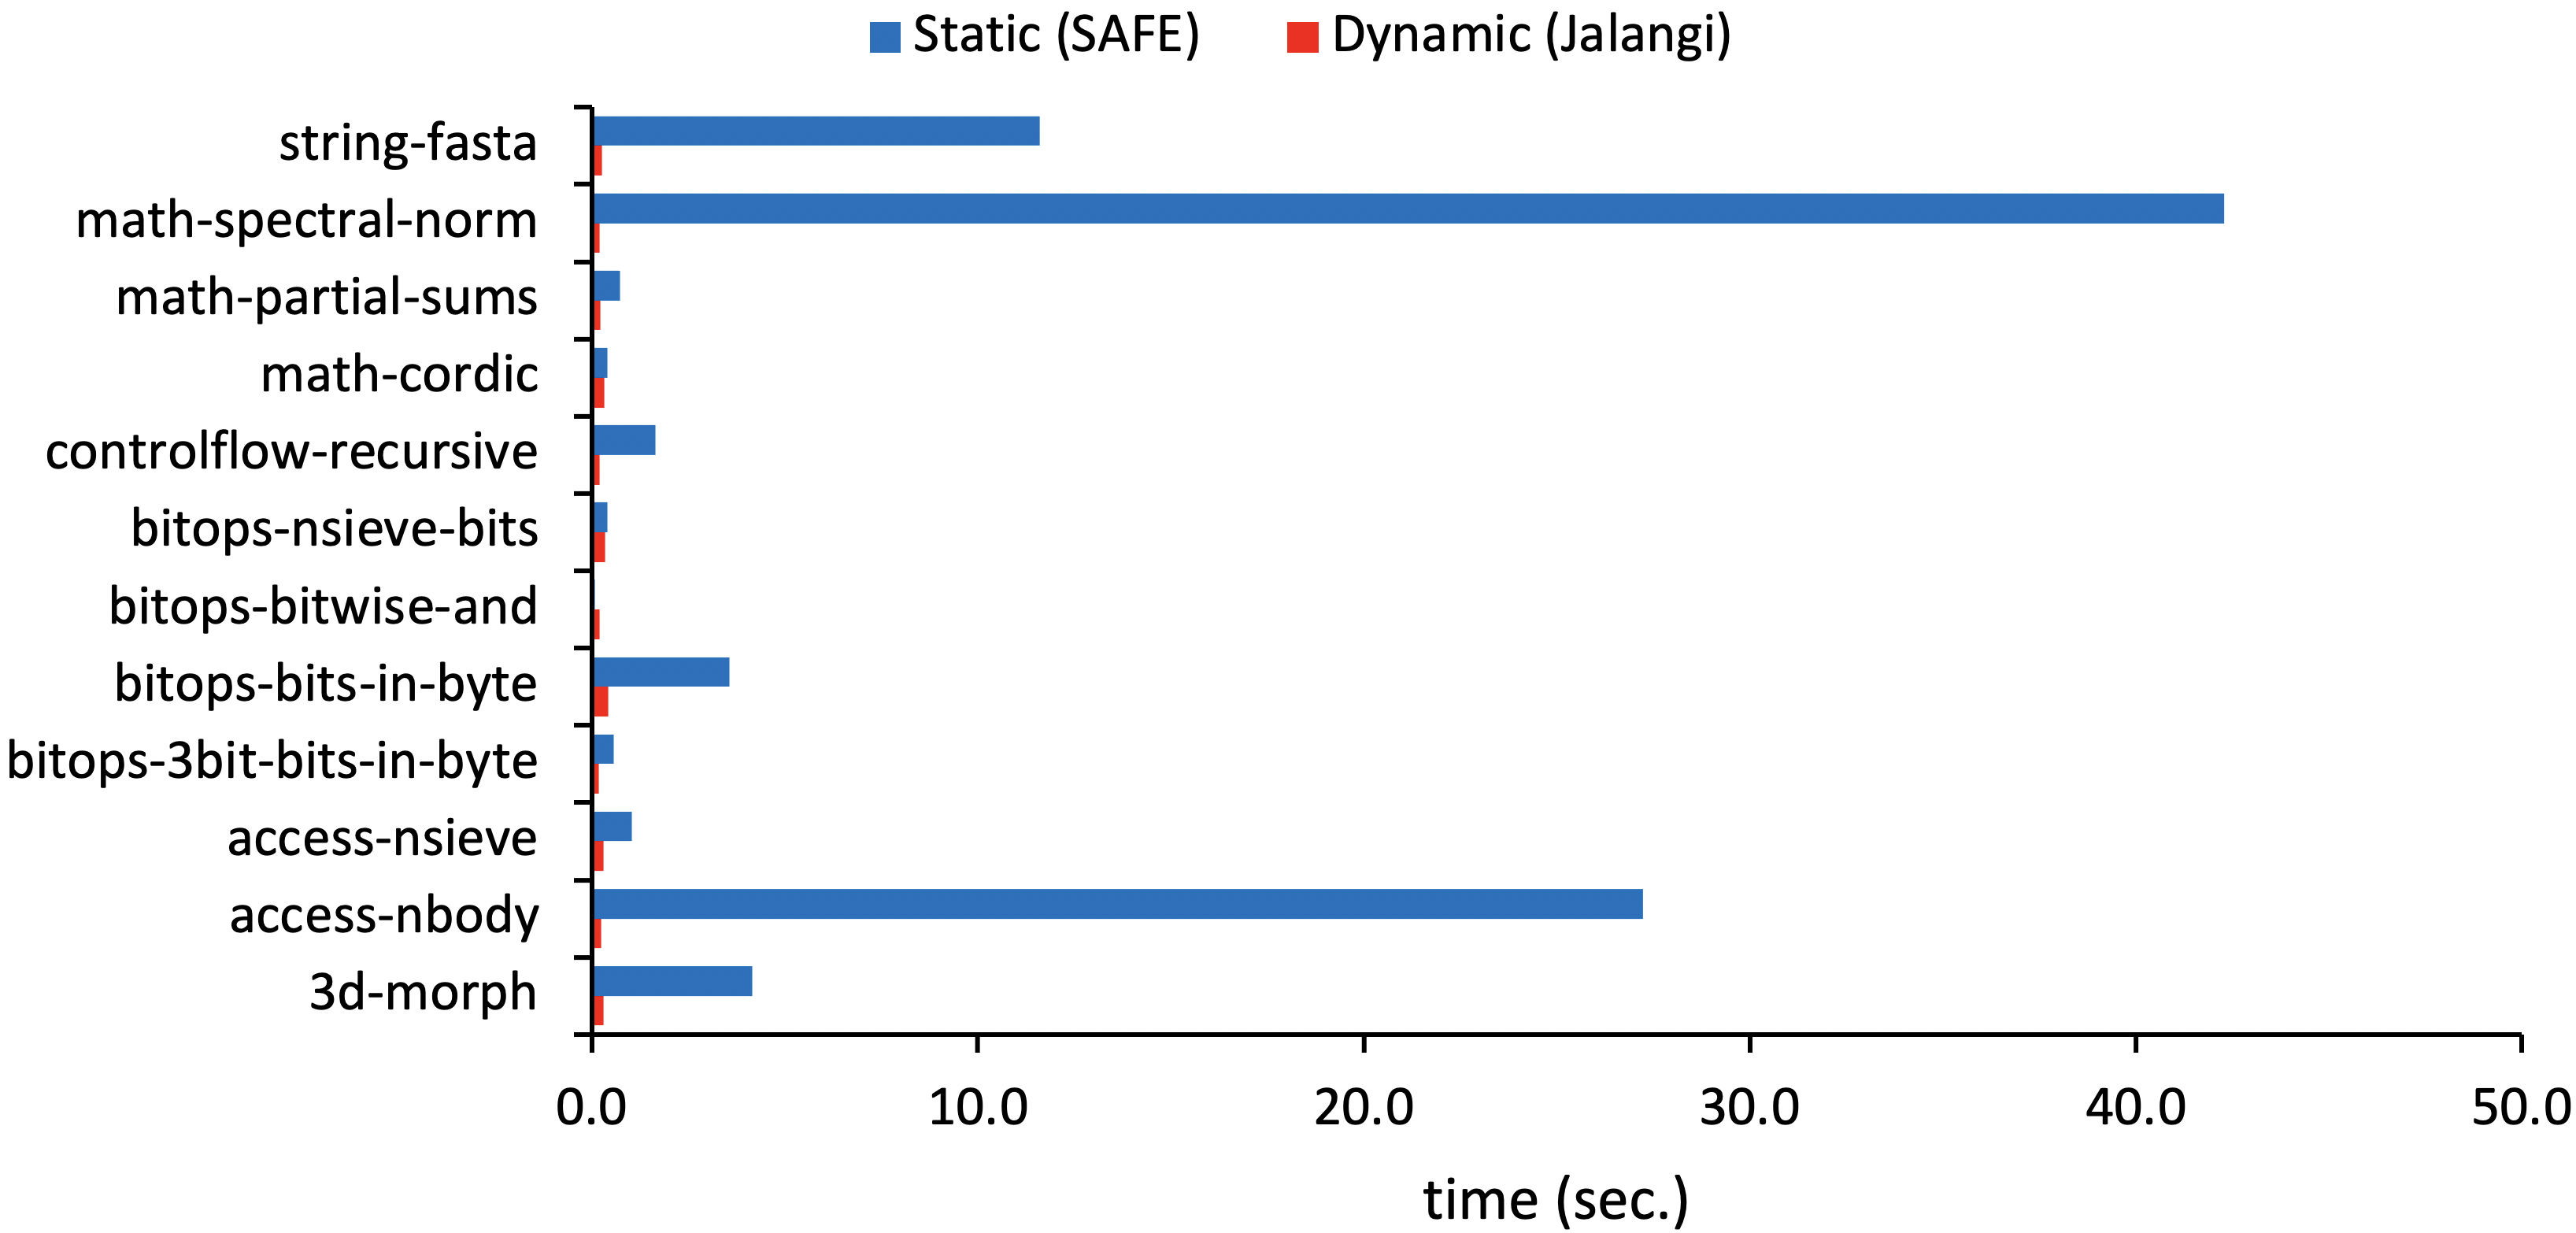
\includegraphics[width=\linewidth]{img/performance_v8v7}
  \vspace*{-2em}
  \caption{The performances of dynamic analysis and static analysis for V8
  benchmarks (version 7)}
  \label{fig:performance}
  \vspace*{-1em}
\end{figure}

Instead of advancing static analysis techniques, several researchers leverage
dynamic analysis to resolve such obstacles in static analysis.  Dynamic
analyzers such as Jalangi~\cite{jalangi} and DLint~\cite{dlint} run on a
highly-optimized commercial JavaScript engine thus they are much faster than
static analysis.  Figure~\ref{fig:performance} shows that the dynamic analysis
(Jalangi) is \inred{X.X}x faster than static analysis (SAFE) for V8 benchmarks
(version 7).  Using high performance dynamic analysis, several researchers
reduce the scope of static analysis~\cite{determinacy, blendedJS}, construct
initial abstract state~\cite{battles, eha}, and automatic modeling of opaque
codes~\cite{sra}.

Unfortunately, existing techniques using dynamic analysis for static analysis
have two limitations: 1) it cannot fully utilize the high performance of dynamic
analysis, and 2) it sacrifices the soundness of static analysis.  Most of
existing techniques are \textit{staged analyses} that first extract specific
information via dynamic analysis and utilize it in static analysis;
\citet{determinacy} identifies determinate expressions that always have the same
value at given program point, \citet{blendedJS} extract the dynamic values to
change expressions as certain literals, and Park et al.~\cite{battles,eha} dump
initial states in a certain host environment or the entry of an event handler.
However, they cannot utilize dynamic analysis any more after starting static
analysis thus they disturb to maximize the performance advantage.  Moreover,
they sacrifice the soundness of static analysis to perform dynamic analysis.
For example, \citet{sra} utilize dynamic analysis for opaque codes with given
abstract arguments during static analysis.  However, they randomly sample finite
concrete values for given abstract arguments when they represent infinite number
of values.  Thus, the analysis result becomes unsound because of the missing
concrete values.

In this paper, we propose a novel \textit{dynamic shortcut} technique to
leverage high performance of dynamic analysis for static analysis by freely
switching between them in a sound way.  Our key observation is that we can
use concrete semantics for specific program parts while preserving the soundness
if they are not dependent with meaning of abstract values.  For example, the
third line of the following program passes the abstract value \jscode{v} stored
in \jscode{obj.p1} to the variable \jscode{x}:
\begin{lstlisting}[style=myJSstyle,numbers=none]
var v = ... // an abstract value
var obj = { p1: v }, y = "p";
x = obj[y + 1];
\end{lstlisting}
Even though \jscode{obj} contains an abstract value \jscode{v}, the semantics of
the third line does not dependent with the meaning of \jscode{v}.  To utilize
this observation in dynamic shortcut, we introduce \textit{sealed symbolic
execution}, which is an augmented concrete execution with sealed symbolic
values.  We represent each abstract value as a sealed symbolic value, which is a
symbolic value that detects when trying to access its actual meaning.  To
evaluate our approach, we implemented $\tool$ by extending the existing
JavaScript static analyzer SAFE with dynamic shortcut.  For evaluation of
$\tool$, we analyzed abstracted versions of \inred{77} official tests of
\inred{Lodash 4} library.

Our contributions in this paper include the following:
\begin{itemize}
  \item We present a novel \textit{dynamic shortcut} for JavaScript static
    analysis to leverage the high performance of dynamic analysis.  We also
    formally define it with sealed symbolic execution and prove the soundness of
    static analysis using dynamic shortcut.
  \item We actualize dynamic shortcut technique in $\tool$, which is an
    extension of an existing JavaScript static analyzer SAFE with a dynamic
    analyzer Jalangi.
  \item For empirical evaluation, we analyzed \inred{77} official tests of
    \inred{Lodash 4} library with randomly abstracted values.  Our tool
    accelerates \inred{X.X}x the static analysis on average.  Moreover, it
    improves \inred{XX.XX}\% of analysis precision by using dynamic shortcut
    instead of manual modeling for \inred{XX.X} opaque functions on average.
\end{itemize}

In the remainder of this paper, Section~\ref{sec:motivation} explains the
motivation of this work with a simple example.  Section~\ref{sec:formal}
formalizes adding dynamic shortcuts on abstract interpretation.  We extended the
formalization with JavaScript specific language features with a core language in
Section~\ref{sec:javascript}.  Section~\ref{sec:implementation} describes
key techniques to implement dynamic shortcuts for JavaScript static analysis.
We describes evaluation result of our techniques with real-world benchmarks in
Section~\ref{sec:eval}.  Section~\ref{sec:related} explains related works and
Section~\ref{sec:conclusion} concludes.
